\def\year{2017}\relax
%File: formatting-instruction.tex
\documentclass[letterpaper]{article} %DO NOT CHANGE THIS
\usepackage{aaai19}  %Required
\usepackage{times}  %Required
\usepackage{helvet}  %Required
\usepackage{courier}  %Required
\usepackage{url}  %Required
\usepackage{graphicx}  %Required
\frenchspacing  %Required
\setlength{\pdfpagewidth}{8.5in}  %Required
\setlength{\pdfpageheight}{11in}  %Required
%PDF Info Is Required:
  \pdfinfo{}
\setcounter{secnumdepth}{0}

\usepackage{amsmath}
\usepackage{amssymb}
\usepackage{amsthm}
\usepackage{multirow}
\usepackage{tikz}
\usetikzlibrary{arrows,automata}
\usepackage{comment}

\usepackage{graphicx}
\usepackage{caption}
\usepackage{subcaption}
\usepackage{listings}

\lstset{
  basicstyle=\ttfamily,
  mathescape
}


\usepackage{multicol}
\usepackage{arydshln}
\usetikzlibrary{calc,backgrounds,positioning,fit}


\newcommand{\tup}[1]{{\langle #1 \rangle}}

\newcommand{\pre}{\mathsf{pre}}     % precondition
\newcommand{\del}{\mathsf{del}}     % effect
\newcommand{\add}{\mathsf{add}}     % effect
\newcommand{\eff}{\mathsf{eff}}     % effect
\newcommand{\cond}{\mathsf{cond}}   % conditional effect
\newcommand{\true}{\mathsf{true}}   % true
\newcommand{\false}{\mathsf{false}} % false
\newcommand{\PE}{\mathrm{PE}}     % precondition
\newcommand{\strips}{\textsc{Strips}}     % precondition


\newtheorem{theorem}{Theorem}
\newtheorem{lemma}[theorem]{Lemma}
\newtheorem{definition}[theorem]{Definition}


\begin{document}

\title{Model Recognition as Planning}

% Commented for blind submission
\author{Diego Aineto\and Sergio Jim\'enez\and Eva Onaindia \and Miquel Ram\'irez\\
{\small Departamento de Sistemas Inform\'aticos y Computaci\'on}\\
{\small Universitat Polit\`ecnica de Val\`encia.}\\
{\small Camino de Vera s/n. 46022 Valencia, Spain}\\
{\small \{dieaigar,serjice,onaindia\}@dsic.upv.es}}



\maketitle
\begin{abstract} 
Given a partially observed plan execution, and a set of possible planning models (models that share the same state variables but that update these variables according to different action models); {\em model recognition} is the task of identifying which model in the set produced/explains the given observation. The paper formalizes the {\em model recognition} task and introduces a novel method to estimate the probability of a \strips\ model to produce an observation of a plan execution. This method, that we called {\em model recognition as planning}, is built on top of off-the-shelf classical planning algorithms and is robust to missing intermediate states and actions in the observation of the plan execution. The effectiveness of {\em model recognition as planning} is shown in a set of \strips\ models encoding different kinds of {\em automata}. We show that {\em model recognition as planning} succeeds to identify the executed automata despite some state variables (e.g. the internal automata state) or the actual applied transitions are unobserved.
\end{abstract}

\section{Introduction}
\label{sec:introduction}
{\em Plan recognition} is the task of predicting the future actions of an agent provided observations of its current behavior~\cite{carberry2001techniques}. {\em Goal recognition} is a closely related task that aims identifying the goals of the observed agent. Goal recognition is considered {\em automated planning} in reverse; while automated planning compute sequences of actions that accounts for a given goals, goal recognition compute goals that account for an observed sequence of actions~\cite{geffner:book:2013}.

Diverse approaches has been proposed for plan/goal recognition such as {\em rule-based systems}, {\em parsing}, {\em graph-covering}, {\em Bayesian nets}, etc~\cite{sukthankar2014plan}. {\em Plan recognition as planning} is the model-based approach for plan/goal recognition that leverages the action model of the observed agent to compute its most likely goal~\cite{ramirez2012plan,ramirez2009plan}.

This paper formalizes the {\em model recognition} task where the object to recognize is not a goal but the {\em planning model} that shapes the behavior of the observed agent. Given a partially observed plan execution, and a set of possible planning models (models that share the same state variables but that update these variables with different action models); {\em model recognition} is the task of identifying the model in the set with the highest probability of producing/explaining the given observation.

\begin{figure}
  \begin{scriptsize}    
  \begin{center}
  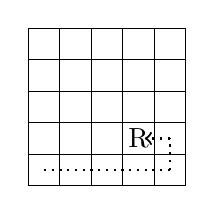
\begin{tikzpicture}[scale=.4]
          \begin{scope}
            \draw (0, 0) grid (5, 5);
            \node[anchor=center] at (3.5, 1.5) {R};
            \node[anchor=center] at (0.5, 0.5) {};
            \draw[thick,style=dotted] (0.5,0.5) -- (4.5,0.5);
            \draw[thick,style=dotted] (4.5,0.5) -- (4.5,1.5);
            \draw[thick,style=dotted,->] (4.5,1.5) -- (3.7,1.5);                        
          \end{scope}
        \end{tikzpicture}
\hspace*{1cm}        
	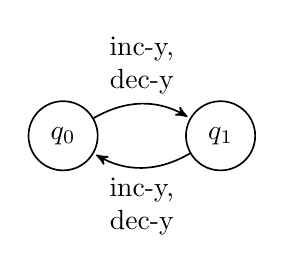
\begin{tikzpicture}[->,>=stealth',shorten >=1pt,auto,node distance=2cm,semithick]
	  \node[state] (A)              {$q_0$};
	  \node[state] (B) [right of=A] {$q_1$};          
	  \path
(A) edge [bend left, align=center] node {inc-y,\\dec-y} (B)
(B) edge [bend left, align=center] node {inc-y,\\dec-y} (A);
	\end{tikzpicture}
  \end{center}
  \end{scriptsize}  
 \caption{\small ({\em Left)} Robot navigating a $5\times 5$ grid. {\em (Right)} Automata to control that the robot only increments its x-coordinate when $q_0$ holds (actions {\tt inc-y} and {\tt dec-y} update the robot y-coordinate and switch the automata state).}
\label{fig:grid-example}
\end{figure}

To better illustrate {\em model recognition}, imagine a robot in a $n\times n$ grid whose navigation is determined by the \strips\ model of Figure~\ref{fig:model-example}. According to this model, the robot can increment its {\em x-coordinate} when {\tt\small $q0$} holds (i.e. at {\em even rows} if {\tt\small $q0$} holds initially) and decrement it when {\tt\small $q1$} holds (at {\em odd rows} if {\tt\small $q0$} holds initially). Apart from this particular navigation model, different action models could be defined within the same state variables (e.g. altering the way {\tt\small $q0$} and {\tt\small $q1$} are required and updated) and these models can determine different kinds of robot navigation. Given an observation of a plan execution (like the one illustrated at Figure~\ref{fig:grid-example}) {\em model recognition} aims to identify the action model that produced/explains that observation, despite relevant information is unobserved (e.g. the applied actions or the value of state variables {\small\tt $q0$} and {\small\tt $q1$}). 

{\em Model recognition} is of interest because once the planning model is recognized, then the model-based machinery for automated planning becomes applicable~\cite{ghallab2004automated}. In addition, it enables identifying different kinds of automata by observing their execution. It is well-known that diverse automata representations, like {\em finite state controllers}, {\em B\"{u}chi automata}, {\em push-down automata}, {\em {\sc GOLOG} programs} or {\em reactive policies}, can be encoded as classical planning models~\cite{baier2007exploiting,Geffner:FSM:AAAI10,patrizi2011computing,ivankovic2015optimal,segovia2017generating}.

The paper also introduces {\em model recognition as planning}; a novel method to estimate the probability of a given \strips\ model to produce an observed plan execution. Our method is built on top of off-the-shelf classical planning algorithms and is robust to missing intermediate states and actions in the observed plan execution. We evaluate the effectiveness of {\em model recognition as planning} with sets of \strips\ models that represent different {\em automata}. All the {\em automata} in a set are defined within the same state variables but different {\em transition functions}. We show that {\em model recognition as planning} succeeds to identify the executed {\em automata} despite some state variables (e.g. the internal automata state) or the actual applied transitions are unobserved.

\begin{figure}
  \begin{tiny}
  \begin{verbatim}
  (:action inc-x
    :parameters (?v1 ?v2)
    :precondition (and (xcoord ?v1) (next ?v1 ?v2) (q0))
    :effect (and (not (xcoord ?v1)) (xcoord ?v2)))

  (:action dec-x
    :parameters (?v1 ?v2)
    :precondition (and (xcoord ?v1) (next ?v2 ?v1) (q1))
    :effect (and (not (xcoord ?v1)) (xcoord ?v2)))

  (:action inc-y-even
    :parameters (?v1 ?v2)
    :precondition (and (ycoord ?v1) (next ?v1 ?v2) (q0))
    :effect (and (not (ycoord ?v1)) (ycoord ?v2)
                 (not (q0)) (q1)))

  (:action inc-y-odd
    :parameters (?v1 ?v2)
    :precondition (and (ycoord ?v1) (next ?v1 ?v2) (q1))
    :effect (and (not (ycoord ?v1)) (ycoord ?v2)
                 (not (q1)) (q0)))

  (:action dec-y-even
    :parameters (?v1 ?v2)
    :precondition (and (ycoord ?v1) (next ?v2 ?v1) (q0))
    :effect (and (not (ycoord ?v1)) (ycoord ?v2)
                 (not (q0)) (q1)))

  (:action dec-y-odd
    :parameters (?v1 ?v2)
    :precondition (and (ycoord ?v1) (next ?v2 ?v1) (q1))
    :effect (and (not (ycoord ?v1)) (ycoord ?v2)
                 (not (q1)) (q0)))
  \end{verbatim}           
  \end{tiny}  
 \caption{\small Example of a \strips\ action model (given in PDDL) for robot navigation in a $n\times n$ grid.}
\label{fig:model-example}
\end{figure}



\section{Background}
\label{sec:background}
This section formalizes the models for {\em classical planning} and for the {\em observation} of the execution of a classical plan.

\subsection{Classical planning}
We use $F$ to denote the set of {\em fluents} (propositional variables) describing a state. A {\em literal} $l$ is a valuation of a fluent $f\in F$, i.e. either~$l=f$ or $l=\neg f$. A set of literals $L$ represents a partial assignment of values to fluents (without loss of generality, we will assume that $L$ does not assign conflicting values to any fluent). We use $\mathcal{L}(F)$ to denote the set of all literal sets on $F$, i.e.~all partial assignments of values to fluents.

A {\em state} $s$ is a full assignment of values to fluents and we explicitly include negative literals $\neg f$ in states; i.e. $|s|=|F|$, so the size of the state space is $2^{|F|}$. Like in PDDL~\cite{fox2003pddl2}, we assume that fluents $F$ are instantiated from a set of {\em predicates} $\Psi$. Each predicate $p\in\Psi$ has an argument list of arity $ar(p)$. Given a set of {\em objects} $\Omega$, the set of fluents $F$ is induced by assigning objects in $\Omega$ to the arguments of predicates in $\Psi$; i.e.~$F=\{p(\omega):p\in\Psi,\omega\in\Omega^{ar(p)}\}$ such that $\Omega^k$ is the $k$-th Cartesian power of $\Omega$.

A {\em classical planning frame} is a $\tup{F,A}$ pair, where $F$ is a set of {\em fluents} and $A$ is a set of {\em actions}. The semantics of actions $a\in A$ is specified with two functions: $\rho(s,a)$ that denotes whether the action $a$ is {\em applicable} in a state $s$ and $\theta(s,a)$ that denotes the {\em successor state} that results of applying the action $a$ in a state $s$. In this work we compactly represent the $\rho$ and $\theta$ functions following the \strips\ model. With this regard, an action $a\in A$ is defined by:
\begin{itemize}
\item $\pre(a)\in\mathcal{L}(F)$, the {\em preconditions} of $a$, is the set of literals that must hold for the action $a\in A$ to be applicable.
\item $\eff^+(a)\in\mathcal{L}(F)$, the {\em positive effects} of $a$, is the set of literals that are true after the application of action $a\in A$.
\item $\eff^-(a)\in\mathcal{L}(F)$, the {\em negative effects} of $a$, is the set of literals that are false after the application of the action.
\end{itemize}
We say that an action $a\in A$ is {\em applicable} in a state $s$ iff $\pre(a)\subseteq s$. The result of applying $a$ in $s$ is the {\em successor state} denoted by $\theta(s,a)=\{s\setminus\eff^-(a))\cup\eff^+(a)\}$.

A {\em classical planning problem} is a tuple $P=\tup{F,A,I,G}$, where $I$ is an initial state and $G\in\mathcal{L}(F)$ is a goal condition. A {\em plan} $\pi$ for $P$ is an action sequence $\pi=\tup{a_1, \ldots, a_n}$ that induces the {\em trajectory} $\tau(\pi,P)=\tup{a_1, s_1, \ldots, a_n, s_n}$ such that $s_0=I$ and, for each {\small $1\leq i\leq n$}, $a_i$ is applicable in $s_{i-1}$ and generates the successor state $s_i=\theta(s_{i-1},a_i)$. The {\em plan length} is denoted with $|\pi|=n$. A plan $\pi$ {\em solves} $P$ iff $G\subseteq s_n$, i.e.,~if the goal condition is satisfied at the last state reached after following the application of the plan $\pi$ in the initial state $I$. A solution plan for $P$ is {\em optimal} if it has minimum length.

\subsection{Conditional effects}
{\em Conditional effects} allow classical planning actions to have different semantics according to the value of the current state. This feature is useful for compactly defining our method for {\em model recognition as planning}. 

An action $a\in A$ with conditional effects is defined as a set of {\em preconditions} $\pre(a)\in\mathcal{L}(F)$ and a set of {\em conditional effects} $\cond(a)$. Each conditional effect $C\rhd E\in\cond(a)$ is composed of two sets of literals $C\in\mathcal{L}(F)$, the {\em condition}, and $E\in\mathcal{L}(F)$, the {\em effect}.

An action $a\in A$ is {\em applicable} in a state $s$ iff $\pre(a)\subseteq s$, and the {\em triggered effects} resulting from the action application are the effects whose conditions hold in $s$:
\[
triggered(s,a)=\bigcup_{C\rhd E\in\cond(a),C\subseteq s} E,
\]

The result of applying action $a$ in state $s$ is the {\em successor} state $\theta(s,a)=\{s\setminus\eff_c^-(s,a))\cup\eff_c^+(s,a)\}$ where $\eff_c^-(s,a)\subseteq triggered(s,a)$ and $\eff_c^+(s,a)\subseteq triggered(s,a)$ are, respectively, the triggered {\em negative} and {\em positive} effects.

\subsection{The observation model}
Given a classical planning problem $P=\tup{F,A,I,G}$ and a trajectory $\tau(\pi,P)$ generated by the execution of a plan $\pi$ that solves $P$; the observation of the execution of $\pi$ on $P$ is $\mathcal{O}(\tau)=\tup{a_1^o,s_1^o \ldots , a_l^o, s_m^o}$, an interleaved combination of {\small $1\leq l\leq |\pi|$} observed actions and {\small $1\leq m\leq |\pi|$} observed states such that:
\begin{itemize}
\item Observed actions are {\em consistent} with $\pi$, which means that $\tup{a_1^o, \ldots, a_l^o}$ is a sub-sequence of $\pi$. 
\item Observed states are a sequence of {\em partial states} $\tup{s_1^o, \ldots, s_m^o}$ that is {\em consistent} with the sequence of states $\tup{s_0, s_1, \ldots, s_n}$ traversed by the trajectory $\tau(\pi,P)$. The initial state $I$ is fully observed while the observed states in $\mathcal{O}(\tau)$ may be partial states, i.e. the value of certain fluents in the intermediate states may not be observed (~$|s_i^o|\leq |F|$ for every $1\leq i\leq m$). Certain states may even be fully unobserved ($0\leq|s_i^o|$ for every $1\leq i\leq m$).  
\end{itemize}

With this regard, we are assuming that a bijective monotone mapping exists between plans and observations~\cite{ramirez2009plan}. We can then  conclude that transiting between two consecutive observed states in $\mathcal{O}(\tau)$ may require the execution of more than a single action ($\theta(s_i^o,\tup{a_1,\ldots,a_k})=s_{i+1}^o$, where ${\small k\geq 1}$ is unknown but finite). In other words, having $\mathcal{O}(\tau)$ does not imply knowing the actual length of $\pi$.

Figure~\ref{fig:grid-example} illustrates the {\em partial observation} of a six-state trajectory \{{\tt\scriptsize<(xcoord 2)(ycoord 1)>, <(xcoord 3)(ycoord 1)>, <(xcoord 4)(ycoord 1)>, <(xcoord 5)(ycoord 1)>, <(xcoord 5)(ycoord 2)>, <(xcoord 4)(ycoord 2)>}\}. In more detail, this observation only contains fluents of the kind {\tt\small (xcoord ?v)} and {\tt\small (ycoord ?v)} because the value of the remaining fluents, namely {\tt\small (next ?v1 ?v2)}, {\tt\small (q0)} and {\tt\small (q1)}, cannot be observed.

\begin{definition}[$\Phi$-observation]
Given a subset of fluents $\Phi\subseteq F$ we say that $\mathcal{O}(\tau)$ is a $\Phi$-observation of the execution of $\pi$ on $P$ iff, for every ${\small 1\leq i\leq m}$, each observed state $s_i^o$ only contains fluents in $\Phi$.
\end{definition}



\section{Model Recognition}
\label{sec:recognition}
The {\em model recognition} task is a tuple $\tup{P,M,\mathcal{O}}$ where:
\begin{itemize}
\item $P=\tup{F,A[\cdot],I,G}$ is a {\em classical planning problem} s.t. the semantics of actions $a\in A[\cdot]$ is unknown (i.e. for each $a\in A[\cdot]$ its corresponding $\rho$ and/or $\theta$ functions are undefined).
\item $M=\{\mathcal{M}_1,\ldots,\mathcal{M}_k\}$ is a non-empty {\em set of k models} for the actions in $A[\cdot]$ s.t., each model in $\mathcal{M}\in M$, defines different function pairs $\tup{\rho,\theta}$ over the state variables $F$.
\item $\mathcal{O}(\tau)$ is an {\em observation} of the execution of an unknown solution plan $\pi$ for the planning problem $P$.
\end{itemize}

{\em Model recognition} can be understood as a {\em classification task} where each class is represented with a different planning model $\mathcal{M}\in M$ and the observed plan execution $\mathcal{O}(\tau)$, is the single example to classify. The planning model associated to each class acts as the corresponding {\em class prototype} and it summarizes any observation of a plan execution that could be synthesized with that model (i.e. the set of all the examples that belong to that class).

We follow the {\em naive Bayes classifier} to assign a model $\mathcal{M}\in M$ to the given observation $\mathcal{O}(\tau)$. Therefore the {\em solution} to the {\em model recognition} task is the subset of models in $M$ that maximizes this expression.
\begin{align}
argmax_{\mathcal{M}\in M} P(\mathcal{O}|\mathcal{M}) P(\mathcal{M}).
\end{align}


\subsection{Formulating the $P(\mathcal{O}|\mathcal{M})$ {\em likelihood}}
The $P(\mathcal{M})$ probability expresses whether one model is known to be a priori more likely than the others. If this probability is not given as input it is reasonable to assume that, {\em a priori}, all models are equiprobable. The challenge in our formulation for {\em model recognition} is the definition of the $P(\mathcal{O}|\mathcal{M})$ {\em likelihood} that expresses the probability of observing $\mathcal{O}(\tau)$ when $\mathcal{M}$ is the planning model.

\begin{figure}
  \begin{scriptsize}
  \begin{center}
	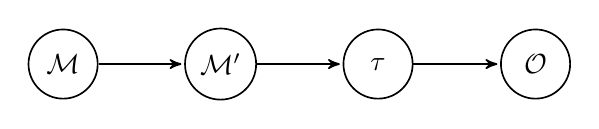
\begin{tikzpicture}[->,>=stealth',shorten >=1pt,auto,node distance=2cm,semithick]
	  \node[state] (A)              {$\mathcal{M}$};
	  \node[state] (B) [right of=A] {$\mathcal{M}'$};
	  \node[state] (C) [right of=B] {$\tau$};
	  \node[state] (D) [right of=C] {$\mathcal{O}$};          
	  \path
(A) edge  node {} (B)
(B) edge  node {} (C)
(C) edge  node {} (D)
;
	\end{tikzpicture}
  \end{center}
  \end{scriptsize}  
 \caption{\small {\em Bayesian network} abstracting that model $\mathcal{M}$ can be {\em transformed} into a model $\mathcal{M}'$ that is able to produce a trajectory $\tau(\pi,P)$ that reaches the goals in $P$ and is consistent with the observation $\mathcal{O}(\tau)$.}
\label{fig:net}
\end{figure}

Our approach to formulate the $P(\mathcal{O}|\mathcal{M})$ {\em likelihood} is to assess the cost of {\em transforming} $\mathcal{M}$ into a model $\mathcal{M'}$ such that: $\mathcal{M'}$ that can produce a trajectory $\tau(\pi,P)$ that reaches the goals in $P$ and is consistent with the observation $\mathcal{O}(\tau)$. Figure~\ref{fig:net} shows the four-variable {\em Bayesian network} abstracting this process. Regarding this network we have the following formulation:
\begin{align}
 P(\mathcal{O}|\mathcal{M})=\sum_{\mathcal{M}'}\sum_{\tau} P(\mathcal{M'}|\mathcal{M})P(\tau|\mathcal{M'})P(\mathcal{O}|\tau),
\end{align}
where $\tau$ ranges over all the trajectories that can be synthesized with a model $\mathcal{M}'$ and $\mathcal{M}'$ ranges over all the models that can be generated {\em transforming} $\mathcal{M}$.

Following this equation, the exact computation of $P(\mathcal{O}|\mathcal{M})$ is intractable. For most planning problems the set of trajectories consistent with an arbitrary observation can easily be huge (infinite in the case of planning problems without dead-ends)~\cite{lesh1995sound}. Even worse, the number of models $\mathcal{M}'$ that can be generated {\em transforming} a given classical planning model $\mathcal{M}$ explodes combinatorially. Instead, our approach is to formulate an effectively estimate of $P(\mathcal{O}|\mathcal{M})$ using the {\em edit distance} referred to \strips\ planning models. {\em Edit distances} are similarity metrics, traditionally computed over {\em strings} or {\em graphs}, and that has been proved successful for {\em pattern recognition}~\cite{masek1980faster,bunke1997relation}. In this work, we assess the cost of {\em transforming} a classical planning model $\mathcal{M}$ into a model $\mathcal{M'}$ formalizing and computing {\em edit distances} that are referred to \strips\ planning models. 


\section{Recognition of \strips\ models}
\label{sec:asPlanning}
Here we analyze the particular instantiation of the {\em model recognition} task where the semantics of actions (i.e. $\rho$ and $\theta$ functions) are specified with \strips\ action schemata. We start formalizing the \strips\ schemata and define the full space of possible \strips\ schemata. Eventually, we introduce an {\em edit distance} for \strips\ schemata to estimate the $P(\mathcal{O}|\mathcal{M})$ likelihoods for classical planning models.

\subsection{Well-defined \strips\ action schemata}
\strips\ action schemata provide a compact representation for specifying classical planning models. Figure~\ref{fig:model-example} shows six \strips\ action schemata, codded in PDDL, that determine a particular kind of robot navigation in $n\times n$ grids.

{\em A \strips\ action schemata} $\xi$ is defined by a list of {\em parameters} $pars(\xi)$, and three list of predicates (namely $pre(\xi)$, $del(\xi)$ and $add(\xi)$) that shape the kind of fluents that can appear in the {\em preconditions}, {\em negative effects} and {\em positive effects} of the actions induced from that schemata.

We say that two \strips\ schemata $\xi$ and $\xi'$ are {\em comparable} iff $pars(\xi)=pars(\xi')$, both share the same list of parameters. For instance, we claim that the six action schemata of Figure~\ref{fig:model-example} are {\em comparable} while, for example, the {\small\tt stack(?v1,?v2)} and {\small\tt pickup(?v1)} schemata from the four operator {\em blocksworld}~\cite{slaney2001blocks} are not. Last but not least, we say that two \strips\ models $\mathcal{M}$ and $\mathcal{M}'$ are {\em comparable} iff there exists a bijective function $\mathcal{M} \mapsto \mathcal{M}^*$ that maps every action schemata $\xi\in\mathcal{M}$ to a comparable schemata $\xi'\in\mathcal{M'}$ and vice versa.

Given a \strips\ action schemata $\xi$ and a set of {\em predicates} $\Psi$ that shape the propositional state variables. The set of FOL interpretations of $\Psi$ over the corresponding parameters of the schemata $\xi$, confines the elements that can appear in the $pre(\xi)$, $del(\xi)$ and $add(\xi)$ lists. We denote this set of FOL interpretations as ${\mathcal I}_{\Psi,\xi}$. For any of the six action schemata defined in Figure~\ref{fig:model-example} the ${\mathcal I}_{\Psi,\xi}$ set contains the same ten elements, ${\mathcal I}_{\Psi,\xi}=${\small\tt\{xcoord($v_1$), xcoord($v_2$), ycoord($v_1$), ycoord($v_2$), q0(), q1(), next($v_1$,$v_1$), next($v_1$,$v_2$), next($v_2$,$v_1$), next($v_2$,$v_2$))\}}.

Despite any element from ${\mathcal I}_{\Psi,\xi}$ can {\em a priori} appear in the $pre(\xi)$, $del(\xi)$ and $add(\xi)$ of a schemata $\xi$, the space of possible \strips\ schemata is constrained by the set ${\mathcal C}$ that includes: 
\begin{itemize}
\item {\em Syntactic constraints}. \strips\ constraints require negative effects appearing as preconditions, negative effects cannot be positive effects at the same time and also, positive effects cannot appear as preconditions. Formally, $del(\xi)\subseteq pre(\xi)$, $del(\xi)\cap add(\xi)=\emptyset$ and $pre(\xi)\cap add(\xi)=\emptyset$). Considering exclusively these syntactic constraints, the size of the space of possible \strips\ schemata is given by $2^{2\times|{\mathcal I}_{\Psi,\xi}|}$. For every action schemata in the navigation model of Figure~\ref{fig:model-example} then $2^{2\times 10}=1,048,576$.
\item {\em Domain-specific constraints}. One can also introduce domain-specific knowledge to more precisely constrain the space of possible schemata. For instance in a {\em robot navigation} model like the one in Figure~\ref{fig:model-example}, {\small\tt q0()} and {\small\tt q1()} are exclusive so they cannot hold at the same time in a $pre(\xi)$/$del(\xi)$/$add(\xi)$ list. Further, {\small\tt next($v_1$,$v_1$)} and {\small\tt next($v_2$,$v_2$)} will not appear at any of these lists because the {\tt\small next} predicate is coding the {\em successor} function for {\em natural numbers}. These domain-specific constraints reduce further the size of the space of possible action schemata to $2^{2\times 7}=16,384$ (for every schemata in the navigation model of Figure~\ref{fig:model-example}).
\end{itemize}

\begin{definition}[Well-defined \strips\ action schemata]
Given a set of {\em predicates} $\Psi$, a list of action {\em parameters} $pars(\xi)$, and set of FOL constraints ${\mathcal C}$ we say that $\xi$ is a {\bf well-defined \strips\ action schemata} iff its three lists $pre(\xi)\subseteq {\mathcal I}_{\Psi,\xi}$, $del(\xi)\subseteq{\mathcal I}_{\Psi,\xi}$ and $add(\xi)\subseteq{\mathcal I}_{\Psi,\xi}$ only contain elements in ${\mathcal I}_{\Psi,\xi}$ and they satisfy all the constraints in ${\mathcal C}$. 
\end{definition}
We say a classical planning action model is {\em well-defined} if all its corresponding  \strips\ action schemata are {\em well-defined}.

\subsection{Edit distances for \strips\ action models}
First, we define the two edit \emph{operations} on a schemata $\xi\in\mathcal{M}$ that belongs to a \strips\ action model $\mathcal{M}\in M$:
\begin{itemize}
\item {\em Deletion}. An element is removed from any of these three lists $pre(\xi)$, $del(\xi)$ and $add(\xi)$ of the operator schemata $\xi\in\mathcal{M}$ such that the resulting schemata is a {\em well-defined} \strips\ action schemata.
\item {\em Insertion}. An element in ${\mathcal I}_{\Psi,\xi}$ is added to any of these three lists $pre(\xi)$, $del(\xi)$ and $add(\xi)$ of the operator schemata $\xi\in\mathcal{M}$ s.t. the resulting schemata is {\em well-defined}.
\end{itemize}

We can now formalize an {\em edit distance} that quantifies how similar two given \strips\ action models are. The distance is symmetric and meets the {\em metric axioms} provided that the two {\em edit operations}, deletion and insertion, have the same positive cost.

\begin{definition}[Edit distance]
  Let $\mathcal{M}$ and $\mathcal{M}'$ be two {\em comparable} and {\em well-defined} \strips\ action models defined within the same set of predicates $\Psi$. The {\bf edit distance} $\delta(\mathcal{M},\mathcal{M}')$ is the minimum number of {\em edit operations} that is required to transform $\mathcal{M}$ into $\mathcal{M}'$.
\end{definition}

Since ${\mathcal I}_{\Psi,\xi}$ are bounded sets, the maximum number of edits that can be introduced to a given action model is bounded as well. The \textbf{maximum edit distance} of a \strips\ model $\mathcal{M}$ built within predicates $\Psi$ is $\delta(\mathcal{M},*)=\sum_{\xi\in\mathcal{M}} 3\times|{\mathcal I}_{\Psi,\xi}|$ (note that, if we consider the syntactic \strips\ constraints, $\delta(\mathcal{M},*)=\sum_{\xi\in\mathcal{M}} 2\times|{\mathcal I}_{\Psi,\xi}|$).

An observation $\mathcal{O}(\tau)$ of the execution of a plan generated with an action model $\mathcal{M}$, reflects {\em semantic knowledge} that constrains further the space of the possible schemata $\xi\in \mathcal{M}$. We talk then about a third kind of constraints, that we call {\em observation constraints}, and that can also be included into the $\mathcal{C}$ set. In addition, {\em observation constraints} allow us to define an edit distance to elicit the $P(\mathcal{O}|\mathcal{M})$ likelihoods. It can be argued that the shorter this  distance the better the given model explains the given observation.

\begin{definition}[Observation edit distance]
  Given $\mathcal{O}(\tau)$, an observation of the execution of a plan for solving $P$ and a \strips\ action model $\mathcal{M}$, defined within the same predicates $\Psi$. The {\bf observation edit distance}, $\delta(\mathcal{M},\mathcal{O})$, is the minimal edit distance from $\mathcal{M}$ to any {\em comparable} and well-defined model $\mathcal{M}'$ s.t. $\mathcal{M}'$ produces a trajectory $\tau(\pi,P)$ that reaches the goals in $P$ and is {\em consistent} with $\mathcal{O}(\tau)$; \[\delta(\mathcal{M},\mathcal{O})=\min_{\forall \mathcal{M}' \rightarrow \mathcal{O}} \delta(\mathcal{M},\mathcal{M}')\]
\end{definition}

The {\em observation edit distance} could also be defined assessing the edition required by the observed plan execution to match the given model. This implies defining {\em edit operations} that modify the observation $\mathcal{O}(\tau)$ instead of $\mathcal{M}$~\cite{yang2007learning,sohrabi:precognition:IJCAI2016}. Our definition of the {\em observation edit distance} is more practical since normally, ${\mathcal I}_{\Psi,\xi}$ is much smaller than $F$ (the number of variables in the schemata should be smaller than the number of objects in a planning problem). In addition, our definition of the {\em observation edit distance} does not accumulate mismatches between the observation and the model that are due to the same source (e.g. the same model flaw).

\begin{definition}[{\em Closest consistent models}] \label{consistent}
Given a model $\mathcal{M}$. The set $M^*$ of {\bf closest consistent models} is the set of action models $\mathcal{M}'$, closest to $\mathcal{M}$ in terms of editions, and that can produce a trajectory $\tau(\pi,P)$ that reaches the goals in $P$ and is {\em consistent} with $\mathcal{O}(\tau)$;
  \[\underset{\forall \mathcal{M}' \rightarrow \mathcal{O}}{\arg\min}\ \delta(\mathcal{M},\mathcal{M}') \]
\end{definition}

\subsection{Approximating the $P(\mathcal{O}|\mathcal{M})$ {\em likelihood}}
Now we we are ready to formulate an effectively estimate of $P(\mathcal{O}|\mathcal{M})$ for the particular instantiation of the {\em model recognition} task where actions are specified with \strips\ schemata.

\subsubsection{Full observability of the executed plan.} The {\em full observability of the executed plan} is a too strong assumption for {\em model recognition} but it allows us to understand how to build a reasonable estimate of the $P(\mathcal{O}|\mathcal{M})$ {\em likelihood} for the general case.

Under the assumption of {\em full observability} there is only a single possible trajectory $\tau^*(\pi,P)$ {\em consistent} with the given observation (because of full observability), so $P(\mathcal{O}|\tau^*)=1$. Further, there is also a single model $M^*$ that can exactly produce that trajectory (otherwise models are identical, at least, in the actions relevant to the observed trajectory so they can be considered the same model).

Provided that there is a single possible trajectory and a single possible model $\mathcal{M}^*$ consistent with the input observation then, the probabilities of expression (2) are not added up and expression (1) simplifies to:
\begin{align}
argmax_{\mathcal{M}\in M} P(\mathcal{M^*}|\mathcal{M}) P(\mathcal{M}).
\end{align}
Note that the term $P(\tau|\mathcal{M^*})$ is taken out of the maximization because is independent of the model $\mathcal{M}\in M$.

\subsubsection{Partial observability of the executed plan.} In a similar way, an approximation of the $P(\mathcal{O}|\mathcal{M})$ {\em likelihood} can be built for the general case where the executed plan is partially observed. To deal with this general scenario we add the following two assumptions:
\begin{enumerate}
\item The {\em principle of rationality}: The expectation that intentional agents will tend to choose actions that achieve their goals most efficiently, given their knowledge of the actual world state~\cite{dennett1983intentional}.
\item {\em The best plans for $P$ are unique or have different cost}.  
\end{enumerate}
Similar assumptions were taken in previous work for {\em goal recognition}~\cite{ramirez2012plan}. They allow us to claim that the sum in equation (2) is dominated by its largest term which corresponds to the shortest trajectory $\tau^*$ (that is assumed to be unique) consistent with the observation, so other terms in the sum are not added up. Again, there is a single model $M^*$ that can produce $\tau^*$. With this regard, both $P(O|\tau^*)$ and $P(\tau^*|\mathcal{M}^*)$ are independent of $\mathcal{M} \in M$ so equation (1) simplifies once again to equation (3) under the previous assumptions.

Note that the more complete is the observation of the plan execution the more accurate is our estimate because it becomes more likely to assume that there is only one plan consistent with the given observation.

\subsubsection{The $P(\mathcal{M^*}|\mathcal{M})$ probability distribution.} $P(\mathcal{M'}|\mathcal{M})$ indicates the probability of {\em transforming} a classical planning model $\mathcal{M}$ into a model $\mathcal{M'}$ by exclusively using the two {\em edit operations} previously defined, {\em deletion} and {\em insertion}.

We know from {\em pattern recognition} that, if string symbols are uniformly random and independent, the distance of a given string to a fixed string follows a {\em Binomial distribution}~\cite{}. Moreover, the probability that a particular string will be within a distance $D$ is the Cumulative Distribution Function (CDF) for the {\em Binomial distribution}~\cite{wilcox1981review}:
\begin{align}
CDF(D)=\sum_{d=0}^D{{N}\choose{d}}  p^d (1-p)^{N-d}
\end{align}
where $N$ is the length of the string, and $p<0.5$ since the cost of applying an {\em edit operation} is higher than do not applying it.

With this regard, and considering that \strips\ models $\mathcal{M}\in M$ can be encoded with a propositional representation of fixed length $N$, we formulate the $P(\mathcal{M'}|\mathcal{M})$ probability distribution mapping the distance $\delta(\mathcal{M},\mathcal{M'})$ according to equation:
\begin{align}
P(\mathcal{M'}|\mathcal{M}) = p^d  (1-p)^{N-d}
\end{align}
where $d=\delta(\mathcal{M},\mathcal{M}')$. Likewise we can formulate $P(\mathcal{M^*}|\mathcal{M})$ with this same equation (5) but instead, the parameter $d$ is given by the {\em observation distance}, $d=\delta(\mathcal{M},\mathcal{O})$.

In other words, we are modeling the edition of a \strips\ planning model as a {\em Bernoulli process} in which there is a sequence of $N$ independent events representing $N$ binary decisions (the $N$ possible applications of the edition operations) such that for every event $P(X=\top)=p$ and $P(X=\perp)=1-p$.



\section{Model Recognition as classical planning}
This section shows that, for \strips\ planning models, $\delta(\mathcal{M},\mathcal{O})$ can be computed (and hence an approximation of the $P(\mathcal{O}|\mathcal{M})$ likelihood) with a a classical planning compilation.

The compilation is an extension of the classical planning compilation for the learning of \strips\ planning models~\cite{aineto2018learning}. The intuition behind this compilation is that a solution to the resulting classical planning task is a sequence of actions that:
\begin{enumerate}
\item {\bf Edits the action model $\mathcal{M}$ to build $\mathcal{M}'$}. A solution plan starts with a {\em prefix} that modifies the preconditions and effects of the action schemata in $\mathcal{M}$ using to the two {\em edit operations} defined above, {\em deletion} and {\em insertion}. 
\item {\bf Validates the edited model $\mathcal{M}'$}. The solution plan continues with a postfix that:
\begin{enumerate}
\item Induces a solution plan $\pi$ for the original classical planning problem $P$.
\item Validates that $\mathcal{O}(\tau)$ is an observation of the execution of $\pi$ on the classical planning problem $P$.
\end{enumerate}
\end{enumerate}

Figure~\ref{fig:plan-pdistance} shows the plan with a prefix (steps [0,6]) for editing the planning model of Figure\ref{fig:model-example} when its schemata {\tt\small inc-x} is defined without preconditions and its positive/negative effects are swapped wrt Figure~\ref{fig:model-example}. The postfix of the plan (steps [7,14]) validates the edited action model at the observation of the plan execution illustrated at Figure~\ref{fig:grid-example}. Note that our interest is not in $\mathcal{M}'$, the edited model resulting from the compilation, but in the number of required {\em edit operations} (insertions and deletions) required by $\mathcal{M}'$ to be validated. In the example of Figure~\ref{fig:plan-pdistance}, $\delta(\mathcal{M},\mathcal{O})=7$.

\begin{figure}
{\tt\tiny
\begin{tabular}{ll}
00 : (insert\_pre\_xcoord\_v1\_inc-x)   & 07 : (validate\_0)\\
01 : (insert\_pre\_next\_v1\_v2\_inc-x) & 08 : (editable\_inc-x 1 2)\\
02 : (insert\_pre\_q0\_inc-x)           & 09 : (editable\_inc-x 2 3)\\
03 : (delete\_del\_xcoord\_v2\_inc-x)   & 10 : (editable\_inc-x 3 4) \\
04 : (delete\_add\_xcoord\_v1\_inc-x)   & 11 : (editable\_inc-x 4 5)\\
05 : (insert\_del\_xcoord\_v1\_inc-x)   & 12 : (editable\_inc-y-even 1 2)\\
06 : (insert\_add\_xcoord\_v2\_inc-x)   & 13 : (editable\_dec-x 5 4)\\
& 14 : (validate\_1)
\end{tabular}
}
 \caption{\small Plan for editing (steps [0-6]) and validating (steps [7-14]) the model of Figure\ref{fig:model-example} when schemata {\tt\small inc-x} has no {\em preconditions} and positive/negative {\em effects} are swapped wrt Figure\ref{fig:model-example}.}
\label{fig:plan-pdistance}
\end{figure}



\subsection{A propositional encoding for \strips\ action schemata}
Given a \strips\ action schemata $\xi$, a propositional encoding for the {\em preconditions}, {\em negative} and {\em positive} effects of that schemata can be represented with fluents of the kind $[pre|del|add]\_e\_\xi$ such that $e\in{\mathcal I}_{\Psi,\xi}$ is a single element from the set of interpretations of predicates $\Psi$ over the corresponding variable names $\Omega_\xi$. Figure~\ref{fig:encoding} shows the propositional encoding for the six action schemata defined in Figure~\ref{fig:model-example}.

The interest of having a propositional encoding for \strips\ action schemata is that, using {\em conditional effects}, it allows to compactly define {\em editable actions}. Actions whose semantics is given by the value of the $[pre|del|add]\_e\_\xi$ fluents at the current state. Given an operator schemata $\xi\in\mathcal{M}$ its {\em editable} version is formalized as:
\begin{small}  
\begin{align*}
\hspace*{7pt}\pre(\mathsf{editable_{\xi}})=&\{pre\_e\_\xi\implies e\}_{\forall e\in{\mathcal I}_{\Psi,\xi}}\\
\cond(\mathsf{editable_{\xi}})=&\{del\_e\_\xi\}\rhd\{\neg e\}_{\forall e\in{\mathcal I}_{\Psi,\xi}},\\
&\{add\_e\_\xi\}\}\rhd\{e\}_{\forall e\in{\mathcal I}_{\Psi,\xi}}.
\end{align*}
\end{small}

Figure~\ref{fig:editable} shows the PDDL encoding of the {\em editable} {\tt\small inc-x(?v1,?v2)} schemata for robot navigation in a $n\times n$ grid (Figure~\ref{fig:model-example}). Note that this editable schemata, when the fluents of Figure~\ref{fig:encoding} hold, behaves exactly as defined in Figure~\ref{fig:model-example}. 

\begin{figure}
\begin{tiny}
\begin{verbatim}
;;; Propositional encoding for inc-x(?v1 ?v2)
(pre_xcoord_v1_inc-x) (pre_next_v1_v2_inc-x) 
(pre_q0__inc-x)
(del_xcoord_v1_inc-x) (add_xcoord_v2_inc-x)

;;; Propositional encoding for dec-x(?v1 ?v2)
(pre_xcoord_v1_dec-x) (pre_next_v2_v1_dec-x) 
(pre_q1___dec-x)
(del_xcoord_v1_dec-x) (add_xcoord_v2_dec-x)

;;; Propositional encoding for inc-y-even(?v1 ?v2)
(pre_ycoord_v1_inc-y-even) (pre_next_v1_v2_inc-y-even)
(pre_q0__inc-y-even)
(del_ycoord_v1_inc-y-even) (del_q0__inc-y-even)
(add_ycoord_v2_inc-y-even) (add_q1__inc-y-even)

;;; Propositional encoding for inc-y-odd(?v1 ?v2)
(pre_ycoord_v1_inc-y-odd) (pre_next_v1_v2_inc-y-odd) 
(pre_q0__inc-y-odd)
(del_ycoord_v1_inc-y-odd) (del_q1__inc-y-odd)
(add_ycoord_v2_inc-y-odd) (add_q0__inc-y-odd)

;;; Propositional encoding for dec-y-even(v1 ?v2)
(pre_ycoord_v1_dec-y-even) (pre_next_v2_v1_dec-y-even)
(pre_q0__dec-y-even)
(del_ycoord_v1_dec-y-even) (del_q0__dec-y-even)
(add_ycoord_v2_dec-y-even) (add_q1__dec-y-even)

;;; Propositional encoding for dec-y-odd(?v1 ?v2)
(pre_ycoord_v1_dec-y-odd) (pre_next_v2_v1_dec-y-odd)
(pre_q1__dec-y-odd)
(del_ycoord_v1_dec-y-odd) (del_q1__dec-y-odd)
(add_ycoord_v2_dec-y-odd) (add_q0__dec-y-odd)
\end{verbatim}
\end{tiny}
 \caption{\small Propositional encoding for the six schemata from Figure~\ref{fig:model-example}.}
\label{fig:encoding}
\end{figure}


\subsection{The compilation formalization}
Conditional effects allow us to compactly define our compilation for computing $\delta(\mathcal{M},\mathcal{O})$ and hence, estimate the $P(\mathcal{O}|\mathcal{M})$ likelihood. Given a \strips\ model $\mathcal{M}\in M$ and the observation $\mathcal{O}(\tau)$ of the execution of a plan for solving $P=\tup{F,A,I,G}$, our compilation outputs a classical planning task with conditional effects $P'=\tup{F',A',I',G'}$:
\begin{itemize}
\item $F'$ extends the original fluents $F$ with:
\begin{itemize}
\item Fluents $[pre|del|add]\_e\_\xi$ to model the possible \strips\ schemata. 
\item The fluents to code the {\em observation constraints}:
\begin{itemize}
\item $F_{\pi}=\{plan(a_i,i)\}_{\small 1\leq i\leq l}$ to code the $i^{th}$ action in $\mathcal{O}(\tau)$. The static facts $next_{i,i+1}$ and the fluents $at_i$, {\small $1\leq i< l$}, are also added to iterate through the $l$ actions in $\mathcal{O}(\tau)$.
\item The fluents $\{test_j\}_{1\leq j\leq m}$, indicating the state observation $s_j\in\mathcal{O}(\tau)$ where the action model is validated.
\end{itemize}
\item The fluents $mode_{edit}$ and $mode_{val}$ to indicate whether the operator schemata are edited or validated.
\end{itemize}
\item $I'$ extends the original initial state $I$ with the fluent $mode_{edit}$ set to true as well as the fluents $F_{\pi}$ plus fluents $at_1$ and $\{next_{i,i+1}\}$, {\small $1\leq i<l$}, for tracking the plan step where the action model is validated. Our compilation assumes that initially $\mathcal{M}'$ is defined as $\mathcal{M}$. Therefore fluents $[pre|del|add]\_e\_\xi$ hold as given by $\mathcal{M}$.

\item $G'=G\bigcup\{at_n,test_m\}$.
\item $A'$ comprises three kinds of actions with conditional effects:
\begin{enumerate}
\item The {\em editable} version of the original actions given by $\mathcal{M}$. This actions have now an extra preconditions because they can only be applied in the {\em validation} mode (i.e. when $mode_{val}$ holds). When the observation $\mathcal{O}(\tau)$ includes observed actions, they also include the extra conditional effects $\{at_{i},plan(a_i,i)\}\rhd\{\neg at_{i},at_{i+1}\}_{\forall i\in [1,l]}$ to validate that actions are applied, exclusively, in the same order as they appear in $\mathcal{O}(\tau)$.\\

\item Actions for {\em editing} operator schemata $\xi\in\mathcal{M}$. This includes the actions for {\em inserting} a new {\em precondition} into an action schemata $\xi\in\mathcal{M}$ and for inserting a new {\em negative} or {\em positive} effect into the action schemata $\xi\in\mathcal{M}$
\begin{small}
\begin{align*}
\hspace*{7pt}\pre(\mathsf{insertPre_{e,\xi}})=&\{\neg pre\_e\_\xi, \neg del\_e\_\xi,\\
& \neg add\_e\_\xi, mode_{edit}\},\\
\cond(\mathsf{insertPre_{e,\xi}})=&\{\emptyset\}\rhd\{pre\_e\_\xi\}.
\end{align*}
\begin{align*}
\hspace*{7pt}\pre(\mathsf{insertEff_{e,\xi}})=&\{\neg del\_e\_\xi, \neg add\_e\_\xi,mode_{edit}\},\\
\cond(\mathsf{insertEff_{e,\xi}})=&\{pre\_e\_\xi\}\rhd\{del\_e\_\xi\},\\
&\{\neg pre\_e\_\xi\}\rhd\{add\_e\_\xi\}.
\end{align*}
\end{small}
Besides these actions, $A'$ also contains the actions for {\em deleting} a {\em precondition} and a negative/positive {\em effect}.

\item Actions for {\em validating} the edited models at the $s_j$ observed states, {\tt\small $0\leq j< m$}.
\begin{small}
\begin{align*}
\hspace*{7pt}\pre(\mathsf{validate_{j}})=&s_j\cup\{test_{j-1}\},\\
\cond(\mathsf{validate_{j}})=&\{\emptyset\}\rhd\{\neg test_{j-1}, test_j,\\
                            &\{mode_{edit}\}\rhd\{\neg mode_{edit}, mode_{val}\}.
\end{align*}
\end{small}
\end{enumerate}
\end{itemize}


\begin{figure}
  \begin{tiny}  
  \begin{verbatim}
(:action editable_inc-x
  :parameters (?v1 ?v2)
  :precondition
    (and (or (not (pre_xcoord_v1_inc-x)) (xcoord ?v1))
         (or (not (pre_xcoord_v2_inc-x)) (xcoord ?v2))
         (or (not (pre_ycoord_v1_inc-x)) (xcoord ?v1))                       
         (or (not (pre_ycoord_v2_inc-x)) (xcoord ?v2))
         (or (not (pre_q0__inc-x)) (q0))
         (or (not (pre_q1__inc-x)) (q1)))
         (or (not (pre_next_v1_v1_inc-x)) (next ?v1 ?v1)))
         (or (not (pre_next_v1_v2_inc-x)) (next ?v1 ?v2)))
         (or (not (pre_next_v2_v1_inc-x)) (next ?v2 ?v1)))
         (or (not (pre_next_v2_v2_inc-x)) (next ?v2 ?v2))))
    :effect (and
       (when (del_xcoord_v1_inc-x) (not (xcoord ?v1)))
       (when (del_xcoord_v2_inc-x) (not (xcoord ?v2)))
       (when (del_ycoord_v1_inc-x) (not (xcoord ?v1)))
       (when (del_ycoord_v2_inc-x) (not (xcoord ?v2)))
       (when (del_q0__inc-x) (not (q0)))
       (when (del_q1__inc-x) (not (q1)))
       (when (del_next_v1_v1_inc-x) (not (next ?v1 ?v1)))
       (when (del_next_v1_v2_inc-x) (not (next ?v1 ?v2)))
       (when (del_next_v2_v1_inc-x) (not (next ?v2 ?v1)))
       (when (del_next_v2_v2_inc-x) (not (next ?v2 ?v2)))
       
       (when (add_xcoord_v1_inc-x) (xcoord ?v1))
       (when (add_xcoord_v2_inc-x) (xcoord ?v2))
       (when (add_ycoord_v1_inc-x) (xcoord ?v1))
       (when (add_ycoord_v2_inc-x) (xcoord ?v2))
       (when (add_q0__inc-x) (q0))
       (when (add_q1__inc-x) (q1))
       (when (add_next_v1_v1_inc-x) (next ?v1 ?v1))
       (when (add_next_v1_v2_inc-x) (next ?v1 ?v2))
       (when (add_next_v2_v1_inc-x) (next ?v2 ?v1))
       (when (add_next_v2_v2_inc-x) (next ?v2 ?v2)))
  \end{verbatim}           
  \end{tiny}  
 \caption{\small Editable version of the {\tt\small inc-x(?v1,?v2)} schemata for robot navigation in a $n\times n$ grid.}
\label{fig:editable}
\end{figure}



\section{Evaluation}
\label{sec:evaluation}
To evaluate the empirical performance of {\em model recognition as planning} we collect a set $M$ of possible \strips\ models, that share the same state variables but define different action models. Then, we randomly choose one of these models $\mathcal{M}\in M$ and use it to produce an observation $\mathcal{O}(\tau)$ of a plan execution. Finally, we follow our {\em model recognition as planning} method to identify the model $\mathcal{M}\in M$ that produced $\mathcal{O}(\tau)$. The experiment is repeated for models of different kind and different observability of the given plan execution.


\subsubsection{Reproducibility.} {\sc Madagascar} is the classical planner we used to solve the instances that result from our compilations for its ability to deal with dead-ends~\cite{rintanen2014madagascar}. Due to its SAT-based nature, {\sc Madagascar} can apply the actions for editing preconditions in a single planning step (in parallel) because there is no interaction between them. Actions for editing effects can also be applied in a single planning step, thus significantly reducing the planning horizon.

The compilation source code, evaluation scripts and benchmarks (including the used training and test sets) are fully available at this anonymous repository {\em } so any experimental data reported in the paper can be reproduced.

\subsubsection{Recognition of {\em Regular Automata}.} In this experiment the models in $M$ represent different {\em regular automata}. Figure~\ref{fig:regautomatae} illustrate a four-symbol four-state {\em regular automata} for recognizing the $\{(abc)^n : n \geq 1 \}$ language. The {\em input alphabet} is $\Sigma=\{a,b,c,\square\}$, and the machine states are $Q=\{q_0,q_1,q_2,\underline{q_3}\}$ (where \underline{$q_3$} is the only acceptor state).

We generated a $M$ set of different \strips\ models that encode different {\em regular automata}. Each $\mathcal{M}\in M$ encodes a different {\em regular automata}. Each automata transition is encoded with a planning action. For instance, the execution of the {\em regular automata} defined in Figure~\ref{fig:regautomatae}, with the sequence of input symbols $abcabc$, produces the following six-action plan {\small $(a,q_0\rightarrow q_1)$, $(b,q_1\rightarrow q_2)$, $(c,q_2\rightarrow q_3)$, $(a,q_3\rightarrow q_1)$, $(b,q_1\rightarrow q_2)$, $(c,q_2\rightarrow q_3)$}.

Here we assume that the actual applied transitions are unknown as well as the internal machine state. Assuming that the actual applied transitions is unknown means that the observation $\mathcal{O}(\tau)$ of the execution of a regular automata contains no actions, it is simply a sequence of states $\mathcal{O}(\tau)=\tup{s_1, \ldots, s_m}$. Assuming that the internal machine state is unknown means that $\mathcal{O}(\tau)$ is a $\Phi$-observation and that the $\Phi$ subset does not contain {\small\tt ($q$)} fluents, with $q\in Q$ and $q\neq q_0$.

\begin{figure}
  \begin{scriptsize}
  \begin{center}
	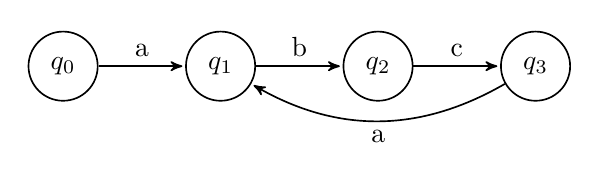
\begin{tikzpicture}[->,>=stealth',shorten >=1pt,auto,node distance=2cm,semithick]
	  \node[state] (A)              {$q_0$};
	  \node[state] (B) [right of=A] {$q_1$};
	  \node[state] (C) [right of=B] {$q_2$};
	  \node[state] (D) [right of=C] {$q_3$};          
	  \path
(A) edge  node {a} (B)
(B) edge  node {b} (C)
(C) edge  node {c} (D)
(D) edge [bend left]  node {a} (B)
;
	\end{tikzpicture}
  \end{center}
  \end{scriptsize}  
 \caption{\small Four-symbol four-state {\em regular automata} for recognizing the $\{(abc)^n : n \geq 1 \}$ language (\underline{$q_3$} is the acceptor state).}
\label{fig:regautomatae}
\end{figure}


\subsubsection{Recognition of navigation models.} In this experiment the given models in $M$ represent different navigation models that are computed as the cross product of a regular automata with a four-operator \strips\ model for navigating a $n\times n$ grid.

In this case the regular automata constrain the applications of the navigation actions producing different navigation policies e.g. like the one in Figure~\ref{fig:model-example}. Given an observation of a plan execution, like the one illustrated at Figure~\ref{fig:grid-example}, here the task is to identify which navigation model produced that observation, despite the the applied actions are unobserved. In addition, for each observed state, only the value of fluents encoding the x and y coordinates of the agent are known while the value of the regular automata conditioning the navigation policy is unknown.

\subsection{Results}




\section{Conclusions}
\label{sec:conclussions}
This paper formalized the {\em model recognition} task and proposed, {\em model recognition as planning}, a method built on top of off-the-shelf classical planning algorithms to estimate the probability of a \strips\ model to produce a partial observation of a plan execution. The paper shows the effectiveness of {\em model recognition as planning} in a set of \strips\ models encoding different kinds of {\em automata}. {\em Model recognition as planning} succeeds to identify the executed automata despite the internal machine state or actual applied transitions, are unobserved.

Previous work on the learning of \strips\ action models also defined semantic error metrics to quantify the errors of a model with respect to the observation of a plan execution~\cite{yang2007learning}. Our approach for quantifying this error is based on the definition of a edit distance for the model which allow us to not accumulate the repetition of errors coming from the the same model flaw. A related approach is recently followed for {\em model reconciliation}~\cite{Kambhampati:mreconciliation:ijcai17} where model edition is used to conform the PDDL models of two different agents. Also  related to this paper is the work on {\em Goal Recognition Design} but in that work the action model is given in advance and fixed~\cite{keren2014goal}.  



%Remarkably, the extension of this piece of work to the FOND planning setting~\cite{muise2012improved} is straightforward by simply considering the {\em all-outcomes} determiniztion of the actions with non-determinitic effects~\cite{yoon2007ff}. An interesting research direction is however to understand how to apply our approach to planning models where the planning models include actions with probabilistic effects~\cite{younes2005first}.  

\bibliographystyle{aaai}
\bibliography{planlearnbibliography}

\end{document}
